\section{Coherence}\label{sec:coh}
% src: F_brief H3 and A11; L3 Sections 0-3, 5, 6 (formation results excluded); L1-P29, L1-X6; L4-P17, L4-P19; L6-P7, L6-C1, L6-C2; L7-P8 to L7-P10, L7-G4, L7-G5, L7-G7, L7-G10; C_critic V7, V8, C4, C5, C8, C9; B5 Sections 3 and 5; C2_check Section 4.2 item 3 and S5; decisions 9, 12, 16, 18

Hypothesis H3 holds that the coherence of message passing is part of the mechanism by which collectives form. To make the claim testable we split coherence into three components, each a property of the edges or cycles of the attention graph. Fidelity is the information about external states that a message carries; calibration is the agreement between the precision a receiver assigns to a message and the message's actual reliability; consistency is the composition of the translations that receivers apply around cycles. None of them is a virtue by itself. A closed group can pass its messages faithfully, find them calibrated by its own agreement and translate them consistently while all its members share a large error about the world, which makes it an echo chamber (\cref{def:mis-echo}). Every coherence statement below is therefore paired with a statement about accuracy.

After the components (\cref{sec:coh-components}) we take calibration (\cref{sec:coh-calibration}) and consistency (\cref{sec:coh-consistency}) in turn, fidelity being treated in the Supplement (\cref{sec:coh-fidelity}), then failures that coherence statistics do not reveal: amplification of belief messages around cycles (\cref{sec:coh-amplification}), domains of incompatible codes (\cref{sec:coh-codes}) and the grounding tension (\cref{sec:coh-tension}); what this contributes to formation is summarized in the Supplement (\cref{sec:coh-formation}). The setting is the linear-Gaussian framework of \cref{sec:fw}: the world $\eta_{t+1}=F\eta_t+w_t$; recognition densities $q_i=\Ncal(m_i,P_i)$ stored as $\mu_i=U_im_i$; messages $T_cU_jm_j+\nu$, read through a code model $\hat H_{ij}$ of the effective code $H_j=T_cU_j$ or through a learned translation $\Theta_{ij}$ of $j$'s internal coordinates, whose true value is $U_iU_j^{-1}$ and whose mistranslation is $\Upsilon_{ij}$ (\cref{def:fw-translation}); the interpretation levels and calibration classes $\mathsf{C0}$, $\mathsf{C1g}$, $\mathsf{C1i}$, $\mathsf{C2}$ of \cref{def:fw-levels,def:fw-calibration}; and the level-0 network of \cref{def:fw-level0}, whose error splits into a common mode and a connected part (\cref{lem:fw-common-mode}). Correlation lengths refer to the connected part, the world-conditional law of \cref{def:col-world-conditional}, and statements about lengths carry the hypothesis labels of \cref{asm:sca-standing}.

\subsection{Three components of coherence, scored with accuracy}\label{sec:coh-components}

We fix a receiver $i$, a sender $j$ that $i$ attends and a round $t$, write $\mathcal I_i$ for the information $i$ holds before the message, its sensory history and the messages already received, and write $\mathcal G_{\mathrm a}=(V,\mathcal E_{\mathrm a})$ for the attention graph, with an edge $j\to i$ when $i$ attends $j$.

\begin{definition}[Components of coherence]\label{def:coh-components}
\begin{enumerate}\renewcommand{\labelenumi}{(\alph{enumi})}
\item Fidelity. The marginal fidelity of the message $y_{ij}$ is $I(\eta_t;y_{ij})$, its receiver fidelity is $I(\eta_t;y_{ij}\mid\mathcal I_i)$, and its believed fidelity is the mutual information between $\eta_t$ and $y_{ij}$ under $i$'s own generative model; at level 0, with code model $\hat H_{ij}$, assigned noise $\hat R_{ij}$ and claimed covariance $\hat P_i$, it is $\frac12\ln\det(I+\hat R_{ij}^{-1}\hat H_{ij}\hat P_i\hat H_{ij}^\top)$. Path versions replace $\eta_t$ by $\eta_{1:t}$.
\item Calibration. Write the messages that $i$ attends as $y_{ij}=\hat H_{ij}\eta_t+\tilde\nu_{ij}$, stack their errors into $\tilde\nu_i$, and let $i$ assign $\tilde\nu_i$ a covariance $\hat R_i$ and a cross-covariance with its prior error $e_i$; at level 0, $\hat R_i$ is block diagonal and the cross-covariance is zero. The assigned precision is marginally calibrated if $\hat R_{ij}=\Cov(\tilde\nu_{ij})$ for every attended $j$; the receiver is calibrated including correlations if $\hat R_i=\Cov(\tilde\nu_i)$ and its assigned cross-covariance is $\Cov(\tilde\nu_i,e_i)$; it is overconfident (underconfident) if its claimed posterior covariance lies below (above) its actual posterior mean-square-error matrix in the Loewner order.
\item Consistency. Let each edge $j\to i$ carry a translation $\Theta_{ij}\in\GL(K)$. A closed walk $\mathfrak c$ is a sequence of agents $i_0,i_1,\dots,i_L=i_0$ with an edge joining $i_{u-1}$ and $i_u$ for every step $u$, and its holonomy $\Hol(\mathfrak c)=\Theta^{(L)}\cdots\Theta^{(1)}$ composes $\Theta^{(u)}=\Theta_{i_ui_{u-1}}$ when step $u$ runs along its edge and $\Theta^{(u)}=\Theta_{i_{u-1}i_u}^{-1}$ when it runs against it. A configuration $\mu=(\mu_i)_{i\in V}$ is in consensus if $\mu_i=\Theta_{ij}\mu_j$ on every edge; these configurations form the consensus space $\mathrm{Cons}(\Theta)$. The translations are consistent on content $v$ at $i_0$ if every holonomy of a closed walk at $i_0$ fixes $v$, and flat if every such holonomy is the identity.
\item Scoring with accuracy. A coherence score of a set $C$ of agents is a pair: a quantity from (a) to (c), aggregated over the edges or cycles inside $C$, and the inaccuracy $\mathcal A_C=\min_{i\in C}\E\Vert m_i-\eta_t\Vert^2_{P_0^{-1}}$ of \cref{def:mis-echo}.
\end{enumerate}
\end{definition}
% src: L3-D1, L3-D2, L3-D4, F_brief H3, critic D5

Receiver fidelity is what an exact receiver extracts from a message and believed fidelity what the receiver thinks it extracts; the gap is the over- or undervaluation of \cref{sec:mis}. The pairing in (d) is forced by a symmetry: an error shared by all agents leaves every statistic of social innovations unchanged (\cref{lem:mis-social-blind}), so only sensory innovations, that is grounding, can certify accuracy. Receiver-side quantities have closed forms for a message $y=H_jm+\nu$ that carries $j$'s posterior mean $m$ of $\eta\sim\Ncal(0,P_0)$, with posterior covariance $P$: then $y=H_j(P_0-P)P_0^{-1}\eta+\nu'$ with $\nu'$ independent of $\eta$ and $\Cov(\nu')=H_j(P-PP_0^{-1}P)H_j^\top+R_c$ (\cref{lem:coh-one-message} in \cref{app:coh-fidelity}, which also gives the fidelity in closed form; checked in \cref{chk:coh-sdpi}). An exactly specified receiver must therefore represent the attenuated code $H_j(P_0-P)P_0^{-1}$ and the sender's estimation noise, both of which the level-0 model omits.

Fidelity decides how far content can travel. Along a Markov chain of jointly Gaussian relays the information about a source is multiplied at each hop by at most the squared top canonical correlation of that hop, and on the infinite ring of scalar level-0 agents the information that an agent's mean carries about the noise injected at a distant agent decays exponentially in their distance at twice the mass, the rate at which influence itself decays, each under the hypotheses stated there (Supplement,\cref{sec:coh-fidelity,prop:coh-relay,prop:coh-info-decay}).

\subsection{Calibration and withdrawal}\label{sec:coh-calibration}

Calibration learned from agreement certifies mutual predictability, not accuracy; the echo chambers that result are treated in \cref{sec:mis} (\cref{thm:mis-echo-chambers,prop:mis-exact-no-echo}). Its second role bears on formation: it decides whether a receiver can register that a sender's messages are mistranslated, and therefore whether inconsistency can move attention. A static model makes every quantity explicit.

\begin{definition}[Static two-group model]\label{def:coh-calibration-model}
The world $\eta\sim\Ncal(0,\sigma_\eta^2I_K)$ is drawn afresh in every round. Agent $j$ senses $s_j=\eta+v_j$, $v_j\sim\Ncal(0,R^s_jI_K)$, and broadcasts its posterior mean $m_j=g_js_j$, $g_j=\sigma_\eta^2/(\sigma_\eta^2+R^s_j)$, in its internal coordinates through the public code $T_c=I_K$ with channel noise $\Ncal(0,R_cI_K)$. Frames $U_j$ and translations $\Theta_{ij}$ are orthogonal, and receiver $i$ carries each message into world coordinates as in \cref{def:fw-translation}, receiving $\tilde y_{ij}=\Upsilon_{ij}m_j+\nu_{ij}$ with the mistranslation $\Upsilon_{ij}=U_i^{-1}\Theta_{ij}U_j$ of \eqref{eq:fw-mistranslation}, which is $I$ exactly when the translation is true; the channel noise, carried into world coordinates by $U_i^{-1}\Theta_{ij}$, is again $\Ncal(0,R_cI_K)$ because $U_i$ and $\Theta_{ij}$ are orthogonal, and we write it $\nu_{ij}$. In the plane $\Upsilon_{ij}=\mathrm{Rot}(\phi_{ij})$, with $\phi_{ij}$ the angle of $\Theta_{ij}$ minus that of $U_iU_j^{-1}$, the translation error of \cref{def:frm-two-group}. Two groups $A$ and $B$ have exact translations within groups and arbitrary orthogonal $\Upsilon_{ij}$ across them. Every receiver senses, attends at most $\kappa$ senders and, at $\gamma=\infty$ and without attention costs, maximizes its believed information about $\eta$, the epistemic part of its expected free energy. Under $\mathsf{C0}$ the likelihood of $\tilde y_{ij}$ does not depend on $\Upsilon_{ij}$; under $\mathsf{C1g}$ and $\mathsf{C1i}$ receiver $i$ models $\tilde y_{ij}$ as $g_j\eta$ plus isotropic noise whose variance $\hat r_{ij}$ matches the second moment of $\tilde y_{ij}-g_j\eta$ on grounded rounds ($\mathsf{C1g}$) or of the innovation $\tilde y_{ij}-g_jg_is_i$ ($\mathsf{C1i}$); under $\mathsf{C2}$ it knows $\Upsilon_{ij}$.
\end{definition}
% src: L3-D7, L3-D8, critic D5 (ladder mapping)

\begin{proposition}[$\mathsf{C0}$ receivers cannot withdraw]\label{prop:coh-c0-blind}
\begin{enumerate}\renewcommand{\labelenumi}{(\alph{enumi})}
\item For a $\mathsf{C0}$ receiver the expected free energy of an attention policy depends on the actual mistranslations only through the receiver's current belief, never through a term for the mistranslation itself.
\item In the static two-group model the believed information of a $\mathsf{C0}$ receiver depends only on claimed covariances, so its expected free energy and its policy posterior over attention sets do not depend on the $\Upsilon_{ij}$ at any policy precision; if its fixed assigned noise depends on a sender only through the sender's sensing noise, it is indifferent between in-group and cross-group senders with equal sensing noise.
\end{enumerate}
\end{proposition}
% src: L3-P14

Blindness has a price. With $\sigma_\eta^2=R^s_j=1$, $R_c=0.1$, $K=2$ and $\kappa=2$, a $\mathsf{C0}$ receiver that attends one in-group sender and one cross-group sender with $\Upsilon=\mathrm{Rot}(\pi)$ has mean-square error $0.708$ per coordinate, against $0.292$ with two in-group senders and $0.500$ from its own sensing alone (\cref{chk:coh-withdrawal}). A calibrated receiver registers mistranslation as noise and acts on it.
% src: L3-E7

\begin{theorem}[Withdrawal under calibration]\label{thm:coh-withdrawal}
In the static two-group model let receiver $i$ be of class $\mathsf{C1g}$ or $\mathsf{C1i}$.
\begin{enumerate}\renewcommand{\labelenumi}{(\alph{enumi})}
\item Its calibrated noise for sender $j$ is $\hat r_{ij}=R_c+g_j^2R^s_j+\hat r^{\mathrm{mt}}_{ij}$ with the mistranslation term $\hat r^{\mathrm{mt}}_{ij}=g_j^2\sigma_\eta^2\Vert\Upsilon_{ij}-I\Vert_F^2/K$ under $\mathsf{C1g}$ and $g_i$ times this under $\mathsf{C1i}$.
\item It attends the $\kappa$ senders with the largest calibrated precisions $\varpi_{ij}=g_j^2/\hat r_{ij}$, ties broken arbitrarily, or all senders if there are fewer than $\kappa$.
\item Let at least $\kappa$ in-group senders be available, with $\kappa$th largest in-group calibrated precision $\varpi^{\mathrm{in}}_{i(\kappa)}$. A cross-group edge $b\to i$ is withdrawn when
\begin{equation}\label{eq:coh-withdrawal}
\hat r^{\mathrm{mt}}_{ib}>\frac{g_b^2}{\varpi^{\mathrm{in}}_{i(\kappa)}}-R_c-g_b^2R^s_b,
\end{equation}
and if the reverse strict inequality holds for some cross-group sender, $i$ attends at least one cross-group sender. Ties aside, the attended graph splits along the cut between $A$ and $B$ if and only if every cross edge satisfies \eqref{eq:coh-withdrawal}. With homogeneous sensing noise every $\Upsilon_{ib}\ne I$ leads to withdrawal.
\end{enumerate}
\end{theorem}
% src: L3-T4; critic V7 (verdict holds, scope stated); attendance clause of (c) corrected: the reverse inequality guarantees some cross sender, not each

The left side of \eqref{eq:coh-withdrawal} is the cost of mistranslation in noise-equivalent units and the right side the information advantage of the cross-group sender. Under $\mathsf{C1i}$ mistranslation is detected only in proportion to the receiver's own sensing gain, so a receiver that does not sense is as blind as a $\mathsf{C0}$ receiver (\cref{lem:mis-social-blind}). The scope is narrow: a static world, infinite policy precision, orthogonal mistranslation, and a $\mathsf{C1}$ model that matches the variance of the mistranslated message but not its correlation with $\eta$. That misspecification is the mechanism. A receiver that knows $\Upsilon_{ij}$, as a $\mathsf{C2}$ receiver does, undoes it and pays no mistranslation cost. In this static model, where the errors of different messages and of the receiver's own sensing are independent given $\eta$, the calibrated model of the corrected message, $g_j\eta$ plus isotropic noise of variance $R_c+g_j^2R^s_j$, is then the exact conditional law, so knowing the translations already gives exact fusion. Withdrawal from inconsistent edges is therefore a calibration-level effect of misreading joint structure; for the dynamic two-group model, where knowing the translation errors falls short of full exact fusion, see the Supplement (\cref{sec:coh-formation}). Bounded-confidence models postulate a withdrawal threshold, which is derived here; those models are discussed in the Supplement (\cref{sec:rel-opinion}). In the dynamic level-0 network the calibrated cost is set by the covariance of the sender's belief with the world (\cref{lem:frm-calibration}). Proofs in \cref{app:coh-calibration}; checks in \cref{chk:coh-withdrawal}.

Withdrawal can fail when a cut separates complementary access to the world: in the instance computed there, a receiver that senses one coordinate keeps attending a mistranslated cross-group sender that senses both (Supplement, \cref{ex:coh-unique-information}).

When translations are learned from grounded rounds on attended edges, persistent inconsistency can sit only on edges attended finitely often (\cref{prop:frm-flattening}), and because attention feeds learning, split and merged configurations can both be stable (\cref{prop:frm-bistability}); these are the first links of the formation chain of \cref{sec:frm}.

\subsection{Consistency}\label{sec:coh-consistency}

Consistency asks whether the translations agents use compose to the identity around cycles; when they do not, no configuration of beliefs agrees on every edge, and the least disagreement that remains measures frustration. Receivers learn their translations of one another independently, so $\Theta_{ji}$ need not be $\Theta_{ij}^{-1}$, and the criterion must hold on directed graphs that are only weakly connected.

\begin{theorem}[Holonomy criterion; (a) is due to \citet{dennis2026magent}]\label{thm:coh-holonomy}
Let the edges of $\mathcal G_{\mathrm a}$ carry translations $\Theta_{ij}\in\GL(K)$ and fix a base agent $i_0$.
\begin{enumerate}\renewcommand{\labelenumi}{(\alph{enumi})}
\item If $\mathcal G_{\mathrm a}$ is strongly connected, $\mu\mapsto\mu_{i_0}$ is a linear bijection from $\mathrm{Cons}(\Theta)$ onto $\bigcap_{\mathfrak c}\mathrm{Fix}(\Hol(\mathfrak c))$, the intersection over the directed closed walks $\mathfrak c$ at $i_0$.
\item If $\mathcal G_{\mathrm a}$ is weakly connected and $\mathcal T$ is a spanning tree of its underlying undirected graph, $\mu\mapsto\mu_{i_0}$ is a linear bijection from $\mathrm{Cons}(\Theta)$ onto $\bigcap_{e\notin\mathcal T}\mathrm{Fix}(\Hol_e)$, where $\Hol_e$ is the holonomy of the closed walk that runs from $i_0$ through $\mathcal T$ to the tail of the non-tree edge $e$, crosses $e$ and returns through $\mathcal T$.
\item Consensus with content $v$ at $i_0$ exists if and only if every $\Hol_e$ fixes $v$, and on strongly connected graphs if and only if every directed closed-walk holonomy at $i_0$ fixes $v$. Full consensus, $\dim\mathrm{Cons}(\Theta)=K$, holds if and only if $\Theta_{ij}=g_ig_j^{-1}$ for some $g_i\in\GL(K)$.
\end{enumerate}
\end{theorem}
% src: L3-T3 (part 1 imported from MAgent Theory 2.0 ch. 17, part 2 new), L6-P7(a,b), L7-G4, critic C8

Partial consensus survives on the common fixed space of the holonomies. When every vector must be fixed, (b) is the balance test of gain graphs on a fundamental system of cycles \citep{zaslavsky1989biased}, read in later restatements; with gains $\pm1$ it is the balance of signed graphs \citep{harary1953notion}, whose two-camp partition \citep{cartwright1956structural} is the simplest inconsistency cut. Part (a) needs return paths: on the acyclic digraph $0\to1$, $1\to2$, $0\to2$ it would claim a $K$-dimensional consensus space, while for generic translations $\mathrm{Cons}(\Theta)=0$, as (b) gives (\cref{chk:coh-holonomy}). Proof in \cref{app:coh-consistency}.

The true translations of agents that encode one world through invertible encodings are flat, so consensus about $\eta$ is always possible in principle, and positive least frustration (\cref{prop:coh-frustration}) arises only from learned translations that differ from the true ones or from agents that do not encode one common world invertibly (Supplement, \cref{prop:coh-flat-true}).

\begin{proposition}[Frustration]\label{prop:coh-frustration}
Give each edge $j\to i$ a precision $\varpi_{ij}>0$ and each agent a positive-definite metric $M_i$, and define the frustration $\mathfrak F(\mu)=\sum_{j\to i}\varpi_{ij}\Vert\mu_i-\Theta_{ij}\mu_j\Vert^2_{M_i}$.
\begin{enumerate}\renewcommand{\labelenumi}{(\alph{enumi})}
\item $\mathfrak F(\mu)=\mu^\top\mathcal L\mu$ with $\mathcal L=\mathcal B^\top\mathcal B\succeq0$, where the incidence operator $\mathcal B$ has, for the edge $j\to i$, the block $\varpi_{ij}^{1/2}M_i^{1/2}$ at $i$ and $-\varpi_{ij}^{1/2}M_i^{1/2}\Theta_{ij}$ at $j$. Its kernel is $\mathrm{Cons}(\Theta)$, and on a weakly connected attention graph $\lambda_{\min}(\mathcal L)$, the least frustration per unit of content, is positive if and only if the holonomies $\Hol_e$ of \cref{thm:coh-holonomy}(b) have no common nonzero fixed vector.
\item On a cycle of $N$ agents, each attending its predecessor, with unit precisions, $M_i=I$ and orthogonal translations whose holonomy has eigenvalues $e^{\mathrm i\theta_1},\dots,e^{\mathrm i\theta_K}$, the spectrum of $\mathcal L$ consists of the numbers $2-2\cos((2\pi u-\theta_r)/N)$, $u=0,\dots,N-1$, $r=1,\dots,K$. If $\phi\in[0,\pi]$ is the smallest modulus of an eigen-angle, $\lambda_{\min}(\mathcal L)=4\sin^2(\phi/(2N))\approx\phi^2/N^2$.
\item Let the translations be orthogonal, $M_i=I$, $\varpi_{ij}\ge\varpi_{\min}$, and $\mathcal T$, $\Hol_e$ as in \cref{thm:coh-holonomy}(b). For each agent $i$ let $\mathcal C_i$ be a nonempty finite family of simple cycles through $i$, with holonomies $\Hol^{(i)}(\mathfrak c)$ based at $i$ and lengths $|\mathfrak c|$, and put $\mathcal D_i=|\mathcal C_i|^{-1}\sum_{\mathfrak c\in\mathcal C_i}|\mathfrak c|^{-1}(I-\Hol^{(i)}(\mathfrak c))^\top(I-\Hol^{(i)}(\mathfrak c))$. Then
\[ \frac{\varpi_{\min}}{N}\min_i\lambda_{\min}(\mathcal D_i)\le\lambda_{\min}(\mathcal L)\le\frac1N\lambda_{\min}\Bigl(\sum_{e\notin\mathcal T}\varpi_e(I-\Hol_e)^\top(I-\Hol_e)\Bigr), \]
and on a single cycle the lower bound is within the factor $\pi^2/4$ of the exact value in (b).
\end{enumerate}
\end{proposition}
% src: L3-P9 (restating MAgent ch. 17 Corollary Frustration, extended to weakly connected graphs through L3-T3), L3-P10, L3-P11, L7-G5

A defect $\phi$ around $N$ agents is spread as $\phi/N$ per edge, so long cycles dilute frustration. With orthogonal translations, $M_i=I$ and $\Theta_{ji}=\Theta_{ij}^{-1}$ on undirected graphs, $\mathcal L$ is, up to normalization, the connection Laplacian of \citet{singer2012vector}, whose spectrum is tied to the frustration of synchronization by a Cheeger-type inequality (Supplement, \cref{sec:rel-sync}); we use none of its constants. Part (a) extends to weakly connected graphs a corollary of \citet{dennis2026magent}, and the lower bound in (c) can be loose by orders of magnitude (\cref{chk:coh-frustration}). Proofs in \cref{app:coh-consistency}.

With rank-limited codes only what is talked about must agree, and coded consensus is the space of global sections of a cellular sheaf, which the holonomy criterion does not characterize (Supplement, \cref{prop:coh-coded}). Under the hypotheses stated there, frustration raises the effective leak of agents that average transported content without sensing (\cref{prop:coh-frustration-grounding}), and cycles on which only edges of small mistranslation are attended have small least frustration whatever their length, although their holonomy can be large (\cref{prop:coh-attended-frustration}). Frustration bounds for translations in $\GL(K)$ are an open problem (\cref{open:coh-frustration-metric}).

\subsection{Amplification by mismatched prior structure}\label{sec:coh-amplification}

A receiver lifts a message into its full belief space and fills the directions the message does not carry from its own prior (\cref{prop:fw-prior-completion}). Composed around a cycle of receivers, these lifts can amplify content even when every code and every translation is correct, a failure that none of the three components registers.

\begin{definition}[Cycle product]\label{def:coh-cycle-product}
Let the $N$ agents of a population form a directed cycle $\mathfrak c$ in which agent $k+1$ receives from agent $k$, indices modulo $N$. Receiver $j$ has prior covariance $P_j\succ0$; sender $i$ has effective code $H_i$ and is read with assigned noise $\hat R_i\succeq0$, with $S_{ji}=H_iP_jH_i^\top+\hat R_i\succ0$. The edge map is the gain-code map $A_{ji}=\Kg_{ji}H_i$, $\Kg_{ji}=P_jH_i^\top S_{ji}^{-1}$, the linear response of the receiver's mean to the sender's mean at level 0; for noiseless codes it is the projector of \cref{prop:fw-prior-completion}(d). The cycle product is $A_{\mathfrak c}=A_{1N}A_{N,N-1}\cdots A_{21}$, and the cycle amplifies when $\rho(A_{\mathfrak c})>1$.
\end{definition}
% src: B5-D4, L4-P19(a), L1-P29(a)

The nonzero spectrum of $A_{\mathfrak c}$ does not depend on where the product starts, and frames enter only by conjugation, since in internal coordinates the edge map is $U_jA_{ji}U_i^{-1}$.

\begin{theorem}[Edge-ratio bound]\label{thm:coh-amplification}
\begin{enumerate}\renewcommand{\labelenumi}{(\alph{enumi})}
\item For an edge $e=(i\to j)$ put $X_{ji}=H_iP_jH_i^\top$, $X_{ii}=H_iP_iH_i^\top$, the edge ratio $\mathfrak r_e=\lambda_{\max}(S_{ji}^{-1}X_{ii})$, and $\mathrm{snr}_e$ through $\mathrm{snr}_e/(1+\mathrm{snr}_e)=\lambda_{\max}(S_{ji}^{-1}X_{ji})$, so that $\mathrm{snr}_e=\lambda_{\max}(\hat R_i^{-1/2}X_{ji}\hat R_i^{-1/2})$ when $\hat R_i\succ0$ and $\mathrm{snr}_e=\infty$ for noiseless codes. Then
\begin{equation}\label{eq:coh-edge-ratio}
\rho(A_{\mathfrak c})\le\prod_{e\in\mathfrak c}\Bigl(\mathfrak r_e\frac{\mathrm{snr}_e}{1+\mathrm{snr}_e}\Bigr)^{1/2}\le\prod_{e\in\mathfrak c}\mathfrak r_e^{1/2},
\end{equation}
so a cycle can amplify only if $\mathfrak r_e>1$ on some edge.
\item If the codes are noiseless and have rank below $K$, a story that leaves agent $1$ returns after $n$ circulations through $\bar A_{\mathfrak c}^n$, with the round-trip map $\bar A_{\mathfrak c}=(I-A_{1N})+A_{\mathfrak c}$, and $\rho(\bar A_{\mathfrak c})=\max\{\rho(A_{\mathfrak c}),1\}$; the story grows geometrically if and only if the cycle amplifies.
\end{enumerate}
\end{theorem}
% src: B5-T2, B5-P16, L1-X6, L4-P19(b,c); decision 9

The edge ratio compares the sender's prior variance in the directions its code carries with the receiver's predictive variance of the message, including the noise the receiver assigns. A cycle can amplify only where the receiver's assigned precision does not account for the sender's own uncertainty, which is a failure of calibration. Proof in \cref{app:coh-amplification}; random cycles never violated either bound, and the sharper one was attained to four digits (\cref{chk:coh-amplification}).

Amplification is excluded by a common prior covariance, by a spread of priors that is small against the assigned noise, by assigned noise that covers the sender's coded uncertainty, and by a common code read with common positive-definite noise, each in the precise form stated there (Supplement, \cref{prop:coh-no-amplification}); explicit amplifying cycles, among them noiseless cycles, for which no spread condition suffices and which amplify at arbitrarily small spread of priors, are in \cref{ex:coh-amplification}.

Amplification does not need misspecified priors: it is a numerical observation that level-0 cycles with codes of rank one still amplify when every prior is the exact posterior of one common prior given private linear-Gaussian data (Supplement, \cref{obs:coh-amplification-information}). Its classification under calibration and the open case of noisy circulation are in \cref{rem:coh-amplification-class,open:coh-amplification-noisy}.

\subsection{Code domains and conformity}\label{sec:coh-codes}

Codes are conventions: which sign, orientation or word a public feature carries. A code is arbitrary in a way a belief about $\eta$ is not, so grounding cannot fix it; what fixes it is the value of being understood, against which stand each agent's idiosyncratic preferences. We derive conformity from expected free energy and bound the size of the domains in which one code holds.

\begin{definition}[Code game]\label{def:coh-code-game}
Agents on an attention graph whose edges are attended in both directions each choose a code $\sigma_i\in\{\pm1\}$ for a public feature, used both to send and to read. On an attended edge, matching codes give a true translation and mismatched codes the mistranslation $-I$ on the feature's coordinates. Receivers are $\mathsf{C1}$-calibrated (\cref{thm:coh-withdrawal}): receiver $i$ assigns isotropic precision $\varpi^{=}$ to a matched message and $\varpi^{\neq}<\varpi^{=}$ to a mismatched one, and holds precision $\Lambda^{\mathrm{own}}$ from its prior and its own sensing. If $i$ has $\mathsf d_i$ partners, $u_i(\sigma)$ of whom use code $\sigma$, its believed information with code $\sigma$ is $\mathcal F_i(u_i(\sigma))$, where
\begin{equation}\label{eq:coh-value}
\mathcal F_i(u)=\frac K2\ln\Bigl(1+\frac{u\varpi^{=}+(\mathsf d_i-u)\varpi^{\neq}}{\Lambda^{\mathrm{own}}}\Bigr),
\end{equation}
with $u$ replaced by $\min\{u,\kappa\}$ and $\mathsf d_i$ by $\kappa$ under a capacity $\kappa<\mathsf d_i$. Each agent also has a pull $h_i$, a prior preference for its native code that enters its expected free energy, so that $G_i(\sigma)=-\mathcal F_i(u_i(\sigma))-h_i\sigma$ up to terms free of $\sigma$.
\end{definition}
% src: L3-D9, B5 Section 3.1, B5-L1

The pull must sit in the expected free energy, not in the habit $E_i$: a habit enters the policy posterior as $\ln E_i$ beside $-\gamma G_i$ and vanishes relative to the couplings as $\gamma\to\infty$. A value affine in $u$ with a slope common to all agents, as in the weak-message limit $\varpi^{=}\ll\Lambda^{\mathrm{own}}$ of \eqref{eq:coh-value}, makes the game pairwise. Away from that limit the value is concave in $u$, and with several features the value an edge loses to mistranslation is concave and subadditive in the number of mismatched features (\cref{lem:coh-c1-value}, in \cref{app:coh-codes}).

No preference for conformity is assumed: with uniform habits the policy posterior gives a logistic adoption rule that is nondecreasing in the local frequency of a code, with an innovation floor at finite policy precision and, for a value affine in $u$ with slope $J$ and no pull, two stable fixed points when $\gamma J\mathsf d_i>2$ (Supplement, \cref{prop:coh-adoption}).

\begin{proposition}[The code game as a potential game]\label{prop:coh-code-potential}
\begin{enumerate}\renewcommand{\labelenumi}{(\alph{enumi})}
\item If $G_i(\sigma)=\sum_jJ_{ij}\mathbf 1[\sigma\ne\sigma_j]-h_i\sigma$ up to terms free of $\sigma$, with symmetric couplings $J_{ij}=J_{ji}\ge0$ on attended edges, then $\Phi_{\mathrm{code}}(\sigma)=\sum_{\{i,j\}}J_{ij}\mathbf 1[\sigma_i\ne\sigma_j]-\sum_ih_i\sigma_i$ is an exact potential, and asynchronous logit revision, in which a uniformly chosen agent resamples its code from $q_i(\sigma)\propto e^{-\gamma G_i(\sigma)}$, is reversible with stationary law proportional to $e^{-\gamma\Phi_{\mathrm{code}}}$, which concentrates on the minimizers of $\Phi_{\mathrm{code}}$ as $\gamma\to\infty$.
\item If every agent has exactly two partners and all agents have the same nondecreasing value $\mathcal F$, the code game is the game of (a) with $J_{ij}=J=\frac12(\mathcal F(2)-\mathcal F(0))$ on every edge.
\item Write $\nabla^{\pm}\mathcal F_i(u)=\mathcal F_i(u+1)-\mathcal F_i(u)+\mathcal F_i(\mathsf d_i-u)-\mathcal F_i(\mathsf d_i-1-u)$ for $u\in\{0,\dots,\mathsf d_i-1\}$. An exact potential exists only if every attended edge $\{i,j\}$ satisfies the following: if $i$ and $j$ have the same other partners, then $\nabla^{\pm}\mathcal F_i(u)=\nabla^{\pm}\mathcal F_j(u)$ for every $u$, and otherwise $\nabla^{\pm}\mathcal F_i$ and $\nabla^{\pm}\mathcal F_j$ do not depend on $u$ and take the same value. Affine values with a common slope satisfy this on every graph, and a common quadratic value on regular graphs, with explicit pairwise potentials. A common value satisfies it on every complete graph, where $\Phi(\sigma)=-\sum_{c=\pm1}\sum_{k=0}^{n_c(\sigma)-1}\mathcal F(k)-\sum_ih_i\sigma_i$, with $n_c(\sigma)$ the number of agents that use code $c$, is an exact potential. For the value \eqref{eq:coh-value}, without capacity and with capacity one, $\nabla^{\pm}\mathcal F_i$ depends on $u$ at every agent with three partners, so a connected attention graph that contains such an agent and is not the complete graph on four agents admits no exact potential, and neither does an open chain of at least three agents.
\end{enumerate}
\end{proposition}
% src: L3-P18, B5-P10 (scope corrected: the ends of an open chain have one partner; affine values need a common slope)

Part (a) is the log-linear learning of \citet{blume1993statistical}, which we know from secondary sources, and by the four-cycle criterion of \citet[Theorem~2.8]{monderer1996potential}, read in the restatement of \citet{arefizadeh2024characterizations}, the condition in (c) is also sufficient. On a ring of four agents with couplings $1$ and $0.3$ in the two directions the logit chain violates detailed balance (\cref{chk:coh-codes}), so asymmetric attention destroys the potential. The code game with a common value is thus an exact potential game on rings and on complete graphs, where it is a congestion game, and on open chains of at least three agents only in its pairwise form. Proof in \cref{app:coh-codes}. For continuous conventions with quadratic conformity to attended partners and to cavity-read group records, the game is again an exact potential game, whose Gibbs precision is diffusive and fixed by the attended couplings, the pulls and the readership, so linear conformity selects no partition that these do not already contain (\cref{prop:hie-conformity}).

\begin{theorem}[One-dimensional code domains]\label{thm:coh-domains-1d}
Let $N\ge3$ agents form a ring, each attending its two neighbors with $\mathsf{C1}$-calibrated reception, let all agents have the same nondecreasing value $\mathcal F$ with $J=\frac12(\mathcal F(2)-\mathcal F(0))>0$, and in (a) and (b) let the pulls $h_1,\dots,h_N$ be the first $N$ terms of a sequence of independent $\Ncal(0,h^2)$ variables, $h>0$.
\begin{enumerate}\renewcommand{\labelenumi}{(\alph{enumi})}
\item Asynchronous logit code dynamics at policy precision $\gamma$ is reversible with stationary law proportional to $e^{-\gamma\Phi_{\mathrm{code}}}$, which concentrates as $\gamma\to\infty$ on the almost surely unique minimizer $\sigma^\ast_N$ of $\Phi_{\mathrm{code}}$, the stochastically stable configuration.
\item The mean domain length $\bar\ell_N$ of $\sigma^\ast_N$, the number of agents divided by the number of maximal runs of one code, satisfies almost surely
\[ \frac12\Bigl(\frac Jh\Bigr)^2\le\liminf_{N\to\infty}\bar\ell_N\le\limsup_{N\to\infty}\bar\ell_N\le26\Bigl(\frac Jh\Bigr)^2+7. \]
\item Without pulls and at finite $\gamma$, two agents at distance $d$ use different codes with probability $\frac12\bigl(1-\frac{\tanh^d(\gamma J/2)+\tanh^{N-d}(\gamma J/2)}{1+\tanh^N(\gamma J/2)}\bigr)$, which tends to $\frac12(1-\tanh^d(\gamma J/2))$ as $N\to\infty$; neighbors then differ with probability $1/(1+e^{\gamma J})$.
\end{enumerate}
\end{theorem}
% src: B5-T1, L3-T5, L3-L3, L3-L4, L3-L5, L3-P18, B5-P10; stated on rings, the chain version holding for the pairwise game

For the $\mathsf{C1}$ value with both partners attended $J=\frac K4\ln\frac{\Lambda^{\mathrm{own}}+2\varpi^{=}}{\Lambda^{\mathrm{own}}+2\varpi^{\neq}}$, and with capacity one $J=\frac K4\ln\frac{\Lambda^{\mathrm{own}}+\varpi^{=}}{\Lambda^{\mathrm{own}}+\varpi^{\neq}}$. Code domains on a ring therefore have a mean length of order the square of the ratio of the believed value lost to mistranslation to the strength of idiosyncratic preference. The scope is binary codes, a common value, asynchronous revision, Gaussian pulls and the stochastically stable state, whose time to be reached is not bounded here; agent-specific values give only a weighted potential game. Part (b) holds for the minimizer of the pairwise potential on an open chain as well, but there (a) needs affine values with a common slope (\cref{prop:coh-code-potential}(c)), and whether code domains have contrast in the sense of \cref{def:col-collective} is open (\cref{open:abs-code-contrast}). \Cref{ex:hie-code-domains} answers this for the declared precision of a belief network on a ring whose attention is cut at the walls between domains, with an answer that depends on the declared geometry, and \cref{conj:hie-conformity-formation} states the formation question that remains: whether the code game with member-written code records and a pragmatic coordination value produces such collectives from a disordered start. The proof (\cref{app:coh-codes}) compares the walls of $\sigma^\ast_N$ with the switches of a greedy hysteresis of the field walk $X_i=h_1+\cdots+h_i$. The constants are not sharp: in exact minimizers on chains of up to $1.5\times10^6$ agents the mean domain length divided by $(J/h)^2$ fell from $4.71$ at $J/h=1$ to $1.06$ at $J/h=32$ (\cref{chk:coh-domains}), and we conjecture that domains and switches agree in number up to one (\cref{conj:coh-walls}), in line with the real-space renormalization of the random-field Ising chain by \citet{fisher2001nonequilibrium}, whose abstract we read. In higher dimension the rigorous results concern random-field models, and their transfer to the code game is conjectural.

Three conjectures carry these questions further (Supplement): in the pairwise game with weak random pulls no code spans a large population in two dimensions while one code does in three or more (\cref{conj:coh-imry-ma}); without pulls the pairwise game on $\Z^2$ coarsens with domain size growing as $t^{1/2}$ (\cref{conj:coh-coarsening}); and a mismatch cost concave in the number of mismatched features makes the walls of different features attract, so that isoglosses, the boundaries of single features, bundle (\cref{conj:coh-bundling}).

\subsection{The grounding tension}\label{sec:coh-tension}

\Cref{asm:int-a11} says that grounding caps the correlation length but makes the collective informative. On a ring of level-0 receivers the trade-off is exact. Each agent senses a scalar world with $0<F<1$ through noise of variance $R^s$ and attends its two neighbors through channels of noise variance $R_c$, assigning precision $\varpi_{\mathrm s}$ to its sensing and $\varpi_{\mathrm y}$ to each message. Its claimed quantities solve $\hat\Lambda^+=1/\hat P^-+\varpi_{\mathrm s}+2\varpi_{\mathrm y}$ and $\hat P^-=F^2/\hat\Lambda^++Q$, its gains are $k^s=\varpi_{\mathrm s}/\hat\Lambda^+$ and $k_{ij}=k^{\mathrm y}=\varpi_{\mathrm y}/\hat\Lambda^+$, and the error-transfer matrix has $W_{ii}=c=F(1-k^s-2k^{\mathrm y})$ and $W_{ij}=a=Fk^{\mathrm y}$ for neighbors, with row sums $\lambda=c+2a=F(1-k^s)=1-\varepsilon$ and local noise variance $q=F^2((k^s)^2R^s+2(k^{\mathrm y})^2R_c)$.

\begin{theorem}[Grounding tension]\label{thm:coh-grounding-tension}
\begin{enumerate}\renewcommand{\labelenumi}{(\alph{enumi})}
\item On the infinite ring with the gains above, \textup{(NN)} and \textup{(C$_r$)} hold with $\lambda=1-\varepsilon<1$, hence \textup{(M)}, and:
\begin{enumerate}\renewcommand{\labelenumii}{(\roman{enumii})}
\item $a/\varepsilon=F\varpi_{\mathrm y}/((1-F)\hat\Lambda^++F\varpi_{\mathrm s})$, and the correlation length of the world-conditional law is $\xi=1/\arccosh(1+\varepsilon/(2a))$ hops. As $F\to1$ at fixed assigned precisions $a/\varepsilon\to\varpi_{\mathrm y}/\varpi_{\mathrm s}$; as $\varpi_{\mathrm y}\to\infty$, $a/\varepsilon\to F/(2(1-F))$ and $\xi\to1/\arccosh(1/F)$, which bounds $\xi$ at every assigned precision.
\item The stationary mean-square error of every agent is
\begin{equation}\label{eq:coh-ring-mse}
\E e_i^2=\frac{Q}{\varepsilon(2-\varepsilon)}+\frac q2\Bigl[\frac{1}{\sqrt{\varepsilon(1-c+2a)}}+\frac{1}{\sqrt{(1+c)^2-4a^2}}\Bigr].
\end{equation}
\item Hence
\begin{equation}\label{eq:coh-tension-law}
\E e_i^2\ge\frac{Q}{\varepsilon(2-\varepsilon)}\ge\frac{Q\xi^2}{2a\cosh^2(1/(2\xi))},
\end{equation}
so that $\E e_i^2\ge(Q/2a)\xi^2(1+O(\xi^{-2}))\ge(Q/F)\xi^2(1+O(\xi^{-2}))$.
\item As $\varpi_{\mathrm y}\to\infty$, $k^s\to0$ and $\E e_i^2\to P_0+F^2R_c/(2\sqrt{1-F^2})>P_0$.
\end{enumerate}
\item In any scalar level-0 network with exact code models satisfying \textup{(Lin)}, \textup{(Loc)}, \textup{(B)} and \textup{(NN)}, with time-invariant $W$, homogeneous sensing gain $k$ and $\lambda=F(1-k)<1$, every agent's stationary mean-square error and the correlation length $\xi$ of the world-conditional law satisfy
\[ \E e_i^2\ge\frac{Q}{1-e^{-2/\xi}}\ge\frac{Q\xi}{2}. \]
\end{enumerate}
\end{theorem}
% src: L3-P19, L3-P20; critic V8 (closed form confirmed to six digits); R3 for the decay rate; 0<F<1, (Loc) and exact codes made explicit

\begin{figure}[t]
  \centering
  % Figure: grounding tension on the level-0 ring (F=0.99, Q=0.02, sensing noise 1, channel noise 0.1).
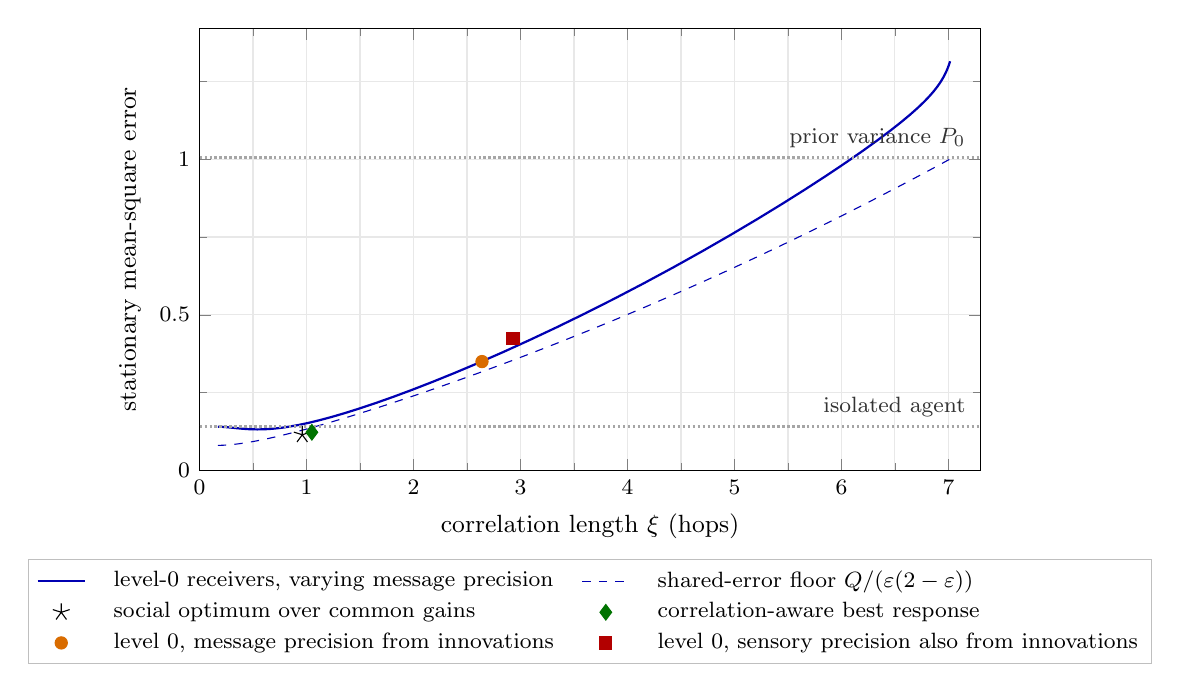
\begin{tikzpicture}
  \begin{axis}[width=11.5cm, height=7.2cm,
      xmin=0, xmax=7.3, ymin=0, ymax=1.42,
      xlabel={correlation length $\xi$ (hops)}, ylabel={stationary mean-square error},
      grid=both, grid style={gray!18}, minor tick num=1,
      legend style={font=\footnotesize, at={(0.5,-0.2)}, anchor=north, draw=gray!50, fill=white, cells={anchor=west}, legend columns=2, column sep=8pt},
      every axis label/.style={font=\small}, tick label style={font=\footnotesize}]
    \addplot[blue!70!black, thick] coordinates {(0.17121,0.14115) (0.17776,0.14107) (0.18483,0.14097) (0.19247,0.14086) (0.20074,0.14071) (0.20973,0.14054) (0.21952,0.14032) (0.23022,0.14006) (0.24194,0.13975) (0.25483,0.13937) (0.26904,0.13893) (0.28474,0.13841) (0.30216,0.13780) (0.32153,0.13712) (0.34312,0.13635) (0.36724,0.13553) (0.39425,0.13468) (0.42451,0.13385) (0.45848,0.13311) (0.49661,0.13256) (0.53941,0.13231) (0.58744,0.13252) (0.64127,0.13335) (0.70153,0.13498) (0.76886,0.13761) (0.84395,0.14143) (0.92749,0.14663) (1.02022,0.15340) (1.12287,0.16193) (1.23620,0.17238) (1.36095,0.18492) (1.49784,0.19973) (1.64754,0.21696) (1.81063,0.23679) (1.98760,0.25939) (2.17875,0.28492) (2.38415,0.31351) (2.60359,0.34528) (2.83650,0.38031) (3.08186,0.41858) (3.33819,0.46002) (3.60343,0.50444) (3.87501,0.55151) (4.14983,0.60077) (4.42437,0.65163) (4.69483,0.70337) (4.95734,0.75520) (5.20820,0.80627) (5.44414,0.85578) (5.66252,0.90301) (5.86148,0.94737) (6.04002,0.98846) (6.19794,1.02605) (6.33578,1.06010) (6.45467,1.09072) (6.55611,1.11813) (6.64184,1.14263) (6.71372,1.16456) (6.77355,1.18425) (6.82307,1.20203) (6.86385,1.21817) (6.89729,1.23292) (6.92463,1.24646) (6.94690,1.25892) (6.96501,1.27038) (6.97971,1.28090) (6.99162,1.29050) (7.00126,1.29919) (7.00905,1.30700) (7.01534,1.31394)};
    \addlegendentry{level-0 receivers, varying message precision}
    \addplot[blue!70!black, dashed] coordinates {(0.17121,0.08093) (0.17776,0.08099) (0.18483,0.08105) (0.19247,0.08113) (0.20074,0.08123) (0.20973,0.08136) (0.21952,0.08152) (0.23022,0.08171) (0.24194,0.08195) (0.25483,0.08224) (0.26904,0.08261) (0.28474,0.08306) (0.30216,0.08361) (0.32153,0.08430) (0.34312,0.08514) (0.36724,0.08618) (0.39425,0.08744) (0.42451,0.08898) (0.45848,0.09085) (0.49661,0.09312) (0.53941,0.09585) (0.58744,0.09912) (0.64127,0.10302) (0.70153,0.10764) (0.76886,0.11308) (0.84395,0.11945) (0.92749,0.12685) (1.02022,0.13541) (1.12287,0.14525) (1.23620,0.15650) (1.36095,0.16927) (1.49784,0.18372) (1.64754,0.19997) (1.81063,0.21816) (1.98760,0.23842) (2.17875,0.26088) (2.38415,0.28563) (2.60359,0.31276) (2.83650,0.34231) (3.08186,0.37425) (3.33819,0.40850) (3.60343,0.44488) (3.87501,0.48312) (4.14983,0.52284) (4.42437,0.56355) (4.69483,0.60467) (4.95734,0.64555) (5.20820,0.68551) (5.44414,0.72391) (5.66252,0.76016) (5.86148,0.79377) (6.04002,0.82442) (6.19794,0.85192) (6.33578,0.87622) (6.45467,0.89740) (6.55611,0.91564) (6.64184,0.93117) (6.71372,0.94428) (6.77355,0.95524) (6.82307,0.96436) (6.86385,0.97190) (6.89729,0.97810) (6.92463,0.98318) (6.94690,0.98732) (6.96501,0.99070) (6.97971,0.99344) (6.99162,0.99567) (7.00126,0.99747) (7.00905,0.99893) (7.01534,1.00011)};
    \addlegendentry{shared-error floor $Q/(\varepsilon(2-\varepsilon))$}
    \addplot[only marks, mark=star, mark size=3.2pt, black] coordinates {(0.96,0.115)};
    \addlegendentry{social optimum over common gains}
    \addplot[only marks, mark=diamond*, mark size=2.8pt, green!45!black] coordinates {(1.05,0.123)};
    \addlegendentry{correlation-aware best response}
    \addplot[only marks, mark=*, mark size=2.2pt, orange!85!black] coordinates {(2.64,0.350)};
    \addlegendentry{level 0, message precision from innovations}
    \addplot[only marks, mark=square*, mark size=2.2pt, red!70!black] coordinates {(2.93,0.425)};
    \addlegendentry{level 0, sensory precision also from innovations}
    \draw[gray!70, densely dotted, thick] (axis cs:0,1.005) -- (axis cs:7.3,1.005);
    \node[font=\footnotesize, gray!40!black, anchor=south east] at (axis cs:7.25,1.005) {prior variance $P_0$};
    \draw[gray!70, densely dotted, thick] (axis cs:0,0.1415) -- (axis cs:7.3,0.1415);
    \node[font=\footnotesize, gray!40!black, anchor=south east] at (axis cs:7.25,0.1415) {isolated agent};
  \end{axis}
\end{tikzpicture}

  \caption{\textbf{The grounding tension on the ring.} Stationary mean-square error of level-0 receivers on a ring against the correlation length $\xi$, as the precision assigned to messages varies ($F=0.99$, $Q=0.02$, sensing noise variance $1$, channel noise variance $0.1$). The dashed curve is the shared-error floor $Q/(\varepsilon(2-\varepsilon))$, which grows like $(Q/2a)\xi^2$. The marks show where agents settle: the social optimum over common gains and the correlation-aware best response sit near $\xi\approx1$, below the error of an isolated agent, while level-0 agents that calibrate message precision from social innovations sit far along the curve, and further still when they calibrate their senses the same way.}
  \label{fig:coh-tension}
\end{figure}

The first term of \eqref{eq:coh-ring-mse} is the shared error, which every agent carries and no agent can see in social innovations; the second is the connected part. On the grid of \cref{chk:coh-grounding} raising the precision on messages lengthens the correlation length, which is checked and not proved in general, while the shared-error floor grows at least quadratically in that length on the ring and at least linearly in any level-0 network with homogeneous grounding. Reach never exceeds its pure-listening limit $1/\arccosh(1/F)$, $7.04$ hops at $F=0.99$, and pure listening drives the error above the prior variance, a strong echo chamber in the sense of \cref{def:mis-echo}. An accuracy target therefore caps the correlation length: on the ring $\xi\lesssim\sqrt{2a\E e_i^2/Q}$. In \cref{fig:coh-tension} the error is smallest at a correlation length of $0.54$ hops, and the closed form agrees to six digits with a direct Lyapunov solution on a ring of 400 agents (\cref{chk:coh-grounding}). Proof in \cref{app:coh-tension}. A record that the members write from their own predictions carries the tension across levels: it slows the correction of an error they share with it (\cref{lem:hie-record-blind}) and raises the shared-error floor, which is nondecreasing in the weight the members give the record (\cref{thm:hie-floor}), and top-down precision assigned above its Kalman value trades disagreement for shared error (\cref{prop:hie-echo-tradeoff}).

Where agents settle on the curve is set by how they assign precision. A level-0 receiver that sets its message precision by minimizing free energy matches a moment that contains no shared error (Supplement, \cref{prop:coh-placement}), and in a numerical observation at the parameters of \cref{fig:coh-tension} such agents settle on the long-$\xi$, low-accuracy side of the social optimum (\cref{obs:coh-placement}); that the myopic equilibrium of correlation-aware agents senses less than the social optimum is conjectured (\cref{conj:coh-externality}).

Read together with the size bound of \cref{cor:col-lstar}, and only as an interpretation because the two bounds are proved in different settings, the tension suggests that large accurate collectives need more than homogeneous local message passing (Supplement, \cref{rem:coh-h4}).

What these results contribute to hypothesis H3, a qualified version in which calibrated receivers of the static two-group model withdraw attention from inconsistent edges under the condition of \cref{thm:coh-withdrawal} while a consistent and mutually calibrated interior can still be an echo chamber, is summarized with the status of the formation chain of \cref{sec:frm} in the Supplement (\cref{sec:coh-formation}).
